\chapter{Emocje - geneza i funkcje}
% \chapter{Emocje w grach - VR w aspekcie neuropsychologicznym}
\label{chap:drugi}



%-------------------------------------------------------
\section{Wprowadzenie}

Emocje towarzyszą człowiekowi w codziennym życiu. Są uważane za uosobienie tego, co czyni nas ludźmi, jednak wydają się być przy tym bardzo podobne do reakcji innych zwierząt na pewne, określone bodźce \citep{website:emotion}.

Sztuka, przemysł rozrywkowy, reklama - wszystkie te dziedziny bazują w dzisiejszych czasach na wywoływaniu emocji u odbiorcy. Każde z tych mediów posiada swoje mocne i słabe strony, jeśli chodzi o wywoływania emocji. Skupiając się na emocjach wywoływanych przez gry, można stwierdzić, że opierają się one na tych samych, sprawdzonych metodach zaczerpniętych z filmów i powieści. Poprzez immersję, gry pozwalają na większe zatracenie się w wirtualnym świecie, co daje możliwość twórcom na wykreowanie unikalnego doświadczenia dla użytkownika, które nie byłoby możliwe do uzyskania używając innych środków przekazu. Gry wideo to wciąż ewoluujące medium, którego potencjał jest nadal badany \citep{button}.

\section{Definicja i klasyfikacja emocji}
Na wstępie należy sklasyfikować i rozróżnić występujące u ludzi stany emocjonalne: afekty, emocje i nastroje. Afekt to ogólny termin, obejmujący szeroki zakres uczuć, których ludzie doświadczają - jest to ogólna koncepcja pokrywająca zarówno emocje i nastroje. Emocja to pojęcie, które jest, ale również było w historii psychologii trudne do zdefiniowania. Poniższa definicja emocji oparta jest głównie o dzieło Frijdy z 1986 roku, czyli jedno z najnowocześniejszych zbiorów badań nad emocjami \citep{oatly}.

``Emocja spowodowana jest zazwyczaj przez świadome lub nieświadome wartościowanie przez podmiot jakiegoś zdarzenia jako istotnego dla jakiejś ważnej dla niego sprawy lub celu; emocja odczuwana jest jako pozytywna, jeżeli zdarzenie sprzyja tej sprawie, a jako negatywna, jeżeli ją utrudnia. Rdzeniem emocji jest gotowość do działania i podsuwanie planów; konkretna emocja nadaje priorytet jednemu lub kilku rodzajom działania, narzucając poczucie ich pilności - może więc zakłócać alternatywne procesy umysłowe lub działania albo rywalizować z nimi. Odmienne typy gotowości tworzą odmienne wyjściowe zarysy relacji z innymi. Konkretna emocja jest zazwyczaj doznawana jako odrębny typ stanu umysłowego, któremu niekiedy towarzyszą lub następują po nim zmiany somatyczne, akty ekspresji i działania'' \citep[s.~95]{oatly}.

Nastroje rozróżniane są od emocji głównie pod względem długości trwania. Pomimo braku definicji typowego czasu jaki trwa emocja bądź nastrój, to nastrój trwa dłużej. Czas trwania stanu afektywnego to nie jedyne kryterium pozwalające na odróżnienie nastrój od emocji. Występowanie specyficznych wyrazów mimicznych przypisywane jest do emocji, natomiast nie są one charakterystyczne dla nastrojów. Nastroje mogą nasilać szansę na wzbudzenie konkretnych emocji - osoba poirytowana może szybciej odczuć gniew, a osoba w pozytywnym nastroju - szczęście. Emocje wynikają najczęściej z relacji człowieka z obiektem - są ukierunkowane, czyli skierowane na dany obiekt, choć można być nieświadomym ich przyczyn - na przykład człowiek może czuć gniew w stosunku do jakiegoś obiektu, choć może być nieświadomym do jakiego konkretnie. Nastrój zaś przypisywany jest jako nieukierunkowany stan afektywny, więc nie jest on skierowany na konkretny obiekt  \citep{ekman}.

Różnica, która wydaje się być najlepszym kryterium w odróżnieniu emocji od nastroju to gotowość do zmiany. Podczas wystąpienia emocji, człowiek wchodzi w stan gotowości na działanie, natomiast podczas wystąpienia nastroju człowiek najczęściej opiera się działaniu, które prowadziłoby do zmiany. Przykładem może być negatywny nastrój, w którym nie przyjmuje się zaproszenia na przyjęcie - przy czym również odrzuca stworzenie stanu, który wydaje się być przyjemniejszym od stanu aktualnego \citep{oatly}.

\section{Proces powstawania emocji}

\subsection{Fazy procesu powstania emocji}
Proces powstawania emocji jest złożony, każda emocja ma swoją przyczynę, przechodzi pewien proces, i rodzi konsekwencje. Emocje w ujęciu Frijdowskim można przedstawić jako ciąg faz zaprezentowany na rysunku \ref{fig:fazes}.

\begin{figure}[h]
	\centering
	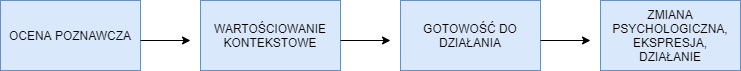
\includegraphics[width=0.9\textwidth]{images/diagram.png}
	\caption{Fazy procesu powstawania emocji.}
	\caption*{Źródło: opracowanie własne na podstawie \citep[s.98]{oatly}.}
	\label{fig:fazes}
\end{figure}

Powstanie emocji u człowieka rozpoczyna się od oceny poznawczej, następnie występuje wartościowanie kontekstowe zdarzenia, które przeobraża się w gotowość do działania. W zależności od emocji i okoliczności, ostatnią fazą jest zmiana psychologiczna, która może, lecz nie musi wystąpić z ekspresją i działaniem \citep{oatly}.

\subsection{Ocena poznawcza}
Jako ocenę poznawczą definiujemy rozpoznanie przez człowieka konkretnego zdarzenia, jako zdarzenia znaczącego dla osiągnięcia celu lub rozwiązania danego problemu. Ocenę poznawczą można podzielić na ocenę pierwotną i ocenę wtórną. Ocena pierwotna dotyczy oceny znaczenia zdarzenia dla danej osoby (zdarzenie bez znaczenia, sprzyjająco-pozytywne lub stresujące) \citep{oatly, website:teoriastresu}. Ocenie pierwotnej według Lazarusa  można przypisać trzy następujące cechy \citep{oatly}:

\begin{enumerate}
\item Ważność zdarzenia dla celu - emocja pojawi się tylko wtedy, kiedy wystąpi okoliczność mająca wpływ na cel lub problem.
\item Zgodność (lub niezgodność) z celem - postęp w osiągnięciu celu wywoła pozytywne emocje, natomiast regres emocje negatywne.
\item Wartość zdarzenia dla podmiotu - przykładem jest zaangażowanie poczucia własnej wartości, które może wywołać dumę lub gniew po zdarzeniu.
\end{enumerate}

Ocena wtórna zaś dotyczy szacowania własnych możliwości i radzenia sobie w sytuacji. Nie zawsze człowiek jest świadomy przyczyny wywołania u niego emocji jak i również faza oceny poznawczej przebiega najczęściej nieświadomie. Ocena czy coś jest ważne dla danego celu lub problemu przebiega mimowolnie w umyśle podmiotu. Aspekty emocji, które są zauważalne, występują w kolejnej fazie \citep{oatly, website:stres}.

\subsection{Wartościowanie kontekstowe}

Podczas doświadczania emocji ważne są również myśli podmiotu, które dotyczą przyszłych planów oraz sposobu w jaki należy poradzić sobie z okolicznościami jakie spowodowały wywołanie emocji. Jeśli w efekcie wywołania emocji, a zatem rezultacie wydarzenia może nastąpić zmiana priorytetów - zdarzenie to musi zostać dogłębnie przeanalizowane. Zatem emocje potrafią znacząco pobudzić aktywność umysłową polegającą między innymi na: zawężeniu uwagi, przywołaniu analogicznych sytuacji z przeszłości w celu skonfrontowania ich z aktualnym problemem czy tworzeniu przyszłych planów. Adaptacja do zmiany przez istoty ludzkie zależy od zrozumienia nowych wydarzeń i poczynaniu planów na podstawie tego co się wydarzyło. Kluczowymi są więc myśli zapoczątkowane emocjami, które decydują o ważności wydarzenia dla podmiotu oraz o tym, jakie należy wykonać działania aby zmienić stan rzeczy na bardziej korzystny. Znaczące jest także wnioskowanie o przyczynie wydarzenia wywołującego emocje, czyli tzw. atrybucja. Właśnie od atrybucji, czyli definiowanych przez ludzi przyczyn wydarzeń zależy charakter i nacechowanie emocji \citep{oatly}.

\subsection{Gotowość do działania}

Człowiek, poczynając od wieku 3 lat jest świadomy, że emocja może stworzyć problem, a co za tym idzie - wymaga działania, które go rozwiąże. Aktywność umysłowa od tego wieku najczęściej wyraża się w pytaniu ``Co z tym zrobić?''. Emocje można przyrównać do ścieżek pośród ludzkich działań. Ukazują to, co jest ważne, pozwalają skupić się na celu lub występującym problemie oraz są motywacją do ewentualnej zmiany biegu wydarzeń, czyli przyszłości - specyficzne emocje nadają priorytety konkretnym działaniom. Najczęściej gotowość do działania oraz plany dotyczą innych ludzi, choć nie jest to reguła. Gotowość do działaia według Frijdy, mówi o tym, że ta wywołana emocjami, będzie zawsze najważniejsza \citep{oatly, teorieemocji}.

\subsection{Ekspresja, zmiany somatyczne, działanie}

Plany, myśli oraz gotowość do działania podmiotu najczęściej są ukryte, ale istnieje sposób na rozpoznanie emocji występujących u ludzi. Najczęściej jest to obserwowane jako chwilowe zakończenie interakcji z otoczeniem przez podmiot, na rzecz interakcji z samym podmiotem, czego przykładem mogą być: napad płaczu, napad śmiechu lub paraliżujący napad strachu \citep{oatly}.

\subsubsection{Ekspresja}

Zakłada się, że emocje są stanami dyskretnymi lecz można je rozpoznać po przypisanej im konkretnej ekspresji - czyli działaniu lub procesie fizjologicznym np. poceniu, łzach. Ekspresja to coś, co zostało uzewnętrznione lub inaczej ``wyrażone'' (ang. expressed). Nie ma uniwersalnych odpowiedników stanów emocjonalnych dla wszystkich społeczeństw - są one kształtowe na różne sposoby dla różnych kultur i grup społecznych. Pomimo tychże różnic, sklasyfikowano pięć grup ekspresji niewerbalnych \citep{oatly}:
\begin{enumerate}
  \item Emblematy - inaczej gesty np. kciuk w górę oznaczający ``wszystko w porządku''. Popularne są również gesty nacechowane negatywnie np. wystawiony środkowy palec lub tzw. gest Kozakiewicza.
  \item Ilustratory - najczęściej połączone z informacjami przekazywanymi werbalnie. Ich intensywność wzrasta wraz ze stopniem pobudzenia emocjonalnego np. machanie rękami, zaciskanie pięści.
  \item Regulatory - przykładem może być kiwanie głową w celu podtrzymania płynności rozmowy.
  \item Przejawy afektu - ekspresje np. uśmiech, podniesienie lub zmarszczenie brwi.
  \item Adaptatory - przejawiają się samopielęgnacją np. dotykanie się po ramionach, co może oznaczać lęk lub konflikt wewnętrzny.
\end{enumerate}

\subsubsection{Zmiany somatyczne}

Jednym ze składników procesu są zmiany somatyczne. Stan somatyczny to: oddech, bicie serca, napięcie mięśni. Część z tych zmian jest wywoływanych podświadomie natomiast można je kontrolować. Oddech można spowolnić, a wykonując odpowiednie ruchy ciała możliwe jest także rozluźnienie mięśni. Dzięki kontrolowaniu zmian somatycznych można zintensyfikować lub osłabić emocje, czego przykładem może być branie wolnych i głębokich wdechów, które mogą wpłynąć na zmniejszenie poczucia lęku lub gniewu \citep{website:samokontrola}.

\subsubsection{Działanie}

Ściśle połączone z emocjami są działania i plany - emocje więc mają silny związek z zachowaniem podmiotu. Dzięki zmianom somatycznym organizm może zacząć wykonywać pewne czynności silniej lub szybciej. Przykładem może być gniew - generuje on zmiany fizjologiczne (pobudzenie pewnych mięśni), co przygotowuje podmiot do działania w szybszy sposób. Emocje jednak nie prowadzą bezpośrednio do zmian motorycznych realizujących konkretne plany, ale mają raczej charakter motywacyjny. Strach na przykład może być motywatorem do uniknięcia straty, tak więc następstwami wystąpienia emocji jest raczej zwiększenie skłonności do wykonania jakiegoś działania, niż samo wykonanie go \citep{ekman}.

\section{Funkcje emocji}

Emocje  lub coś ekwiwalentnego do nich są istotne dla złożonych, inteligentnych systemów, które mają różne motywy i działają w złożonym środowisku - nie tylko dla istot ludzkich. Są one ważne w otoczeniu, które nie jest w pełni poznane i nie jest możliwa jego pełna kontrola \citep{oatly}.

Emocje służą więc do uświadamiania podmiotowi jego aktualnego położenia w świecie i zaistniałej sytuacji, lecz nie są narzędziem, które przystosuje ten podmiot do bieżącej sytuacji. Tak więc można wywnioskować, że służą one adaptacji, ale funkcja ta nie jest wykorzystywana przy każdym przejawie wystąpienia emocji. Tak więc występujące emocje możemy sklasyfikować jako funkcjonalne oraz niefunkcjonalne \citep{ekman}.

Odczuwanie pozytywnych emocji ma charakter wzmocnienia - sygnalizują, że aktualnie wykonywane działania przybliżają jednostkę do osiągnięcia celu i motywują do kontynuacji tychże działań. Negatywne zaś wzbudzane są poprzez zdarzenia zagrażające osiągnięciu celów. Informują o  nieodzowności podjęcia konkretnych działań mających na celu zmianę aktualnego (złego) stanu rzeczy albo powstrzymują nadchodzące ewentualne nieprzychylne zmiany \citep{ekman}.

Innymi słowy emocje służą podtrzymaniu lub zmianie pewnych powiązań podmiotu z jego otoczeniem - nie są więc ukierunkowane na samo otoczenie. W dodatku emocje mogą regulować zasoby energii, które są wydawane w interakcji podmiotu z środowiskiem np. apatia towarzysząca smutkowi ułatwia przeżycie negatywnych wydarzeń w życiu poprzez zmniejszenie wrażliwości na doświadczanie bodźców emocjonalnych \citep{ekman}.

Kolejną funkcją emocji jest regulacja kontaktów społecznych, czyli innymi słowy regulacja zachowań pozwalająca na poprawne życie w społeczeństwie. Świadomość, że jakieś działanie może wywołać uczucie wstydu, może doprowadzić do pohamowania jego realizacji. Podobną, ale bardziej ogólną funkcje pełni wywołanie poczucia winy, które pozwala na uniknięcie kary za przewinienia \citep{ekman}.

Niektóre z przejawów emocji nie pełnią żadnej funkcji oraz zdają się być szkodliwe. Najlepszym przykładem zdają się być tęsknota i smutek. Czynią one życie bogatszym oraz skłaniają do refleksji, ale nie posiadają konkretnej funkcji. Emocje mimo to należy uznać za pożyteczny mechanizm, ale nie oznacza to, że każdy przejaw emocji jest użyteczny \citep{ekman}.
